% ============================================================
%  MODULO 16 — Atlas Visual Didatico: mapas por elemento e arquitetura
%  SPEC R680 — 10 fluxogramas TikZ, sem novos pacotes
%  NotebookLM consultado em 05/10/2026: notebook_list ok (225);
%  notebook_create bloqueado sem confirmacao explicita do operador.
% ============================================================
\chapter{Atlas Visual: Cada Elemento em Um Mapa}

\roteirodidatico
{Ana se orienta por figuras; Bruno confere por setas. Este atlas traduz cada arquitetura do livro em um mapa de uma pagina: caixas sao lugares ou decisoes, setas sao caminhos ou devolucoes.}
{\emph{Mapa} mostra territorios; \emph{fluxograma} mostra ordem; \emph{diagrama} mostra relacoes. \emph{Losango} e decisao; \emph{retangulo duplo} e ponto de partida ou chegada.}
{Siga cada mapa com o dedo: de onde parte, por onde passa, onde pode voltar. Depois abra o arquivo indicado e confira se o caminho existe no codigo.}
{Mapa resume relacoes principais, nao todas as chamadas. Modelo explicativo nao e pipeline universal nem prova de desempenho.}
{Para o elemento que voce estuda, que caixa o contem, que seta o liga e que registro prova que o caminho foi percorrido?}

\casoguiado{como usar este atlas}
{Ana abre o mapa M9 e conta a propria historia em quatro casas: funcional, estrutural, teorica e reproducao. Bruno abre o mapa M5 e executa cada losango como teste: passou, segue; reprovou, volta. Quando discordam, o mapa decide o que conferir, nao quem tem razao.}

\section{Mapas mestres: a casa inteira}

\elemento{Como ler cada mapa}{\metainfo{ID}{ATLAS-LEIT} \hfill \metainfo{Regra}{dedo antes do terminal}}

\begin{descricao}
Todo mapa deste capitulo usa as mesmas formas: retangulo simples e etapa, retangulo escuro e marco, losango e decisao com saida sim ou nao, seta cheia e fluxo, seta tracejada e retorno de aprendizado. A legenda vale para os dez mapas.
\end{descricao}

\begin{flowch}[M1 -- Mapa mestre das 8 camadas]{fonte: mod-02 e MAPA ECOSSISTEMA COMPLETO}
\matrix[matrix of nodes,name=m1,row sep=2.2mm,column sep=2.5mm,nodes={fn},ampersand replacement=\&]{
 |[fns]|7 Aplicacoes: skills, livros, pesquisa \\
 |[fns]|6 Integracoes: MCP e executores \\
 |[fns]|5 Evolucao: specs, ciclos, corrigendum \\
 |[fne]|4 Qualidade: SDD e TDD com gate \\
 |[fne]|3 Orquestracao: roteador e atencao \\
 |[fns]|2 Memoria: Quadro e MetaBus \\
 |[fns]|1 Interfaces: CLI e catalogo \\
 |[fns]|0 Fundacao: principios e infra \\
};
\draw[seta] (m1-1-1.south)--(m1-2-1.north);
\draw[seta] (m1-2-1.south)--(m1-3-1.north);
\draw[seta] (m1-3-1.south)--(m1-4-1.north);
\draw[seta] (m1-4-1.south)--(m1-5-1.north);
\draw[seta] (m1-5-1.south)--(m1-6-1.north);
\draw[seta] (m1-6-1.south)--(m1-7-1.north);
\draw[seta] (m1-7-1.south)--(m1-8-1.north);
\end{flowch}

\begin{descricao}
Leitura funcional: de fora, entra pedido e sai resposta com fonte. Leitura estrutural: camadas 1 a 3 atendem e roteiam; 2 guarda; 4 barra; 6 chama fora. Codigo: \pth{marceloclaro/orchestrator.py}, \pth{mci/}, \pth{trust/}, \pth{opencode.json}. Limite: seta aqui e dependencia principal, nao unica possivel.
\end{descricao}

\begin{flowch}[M2 -- Ciclo de orquestracao]{fonte: marceloclaro/orchestrator.py}
\matrix[matrix of nodes,name=m2,row sep=5mm,column sep=4mm,nodes={fn},ampersand replacement=\&]{
 |[fne]|PERCEBE \& |[fne]|DELEGA \& |[fne]|EXECUTA \& |[fne]|REFLETE \\
};
\draw[seta] (m2-1-1)--(m2-1-2);
\draw[seta] (m2-1-2)--(m2-1-3);
\draw[seta] (m2-1-3)--(m2-1-4);
\draw[seta,bend right=30] (m2-1-4) to node[below,font=\tiny]{retorno ao MetaBus} (m2-1-1);
\end{flowch}

\begin{descricao}
Ana ve um balcao unico que nunca divide sem anotar. Bruno ve quatro funcoes encadeadas com retorno gravado. Sem a seta de baixo, seria fila; com ela, e ciclo com aprendizado.
\end{descricao}

\section{Coordenacao e memoria}

\begin{flowch}[M3 -- Quadro Negro A2A]{fonte: protocolo Blackboard A2A}
\matrix[matrix of nodes,name=m3,row sep=4mm,column sep=4mm,nodes={fn},ampersand replacement=\&]{
 |[fn]|Tarefa com criterio \& |[fne]|Orquestrador \& |[fn]|Quadro Negro \\
 |[fn]|Agente busca \& |[fn]|Agente resume \& |[fn]|Agente revisa \\
};
\draw[seta] (m3-1-1)--(m3-1-2);
\draw[seta] (m3-1-2)--(m3-1-3);
\draw[seta] (m3-1-3.south)--(m3-2-2.north);
\draw[seta] (m3-2-1)--(m3-2-2);
\draw[seta] (m3-2-2)--(m3-2-3);
\end{flowch}

\begin{descricao}
O Orquestrador publica a chamada, agentes voluntariam-se por capacidade, o Quadro registra dono de cada parte. Rastro: entradas do Quadro com tarefa, candidato, escore e decisao.
\end{descricao}

\begin{flowch}[M4 -- Memoria e MetaBus]{fonte: mci/}
\matrix[matrix of nodes,name=m4,row sep=3mm,column sep=4mm,nodes={fn},ampersand replacement=\&]{
 |[fns]|Execucao \& |[fn]|Episodica: o que aconteceu \\
 |[fns]|Reflexao \& |[fn]|Semantica: licao extraida \\
 |[fne]|Proxima tarefa \& |[fn]|MetaBus: contexto carregado \\
};
\draw[seta] (m4-1-1)--(m4-1-2);
\draw[seta] (m4-1-2.south)--(m4-2-2.north);
\draw[seta] (m4-2-1)--(m4-2-2);
\draw[seta] (m4-2-2.south)--(m4-3-2.north);
\draw[seta] (m4-3-1)--(m4-3-2);
\end{flowch}

\begin{descricao}
Fazer gera episodio; refletir extrai licao; lembrar carrega contexto. Sem caderno, cada pedido comeca do zero; com ele, erro vira criterio.
\end{descricao}

\section{Qualidade e roteamento}

\begin{flowch}[M5 -- SDD e TDD com gate fechado]{fonte: sdd/spec\_engine.py e trust/}
\matrix[matrix of nodes,name=m5,row sep=3mm,column sep=4mm,nodes={fn},ampersand replacement=\&]{
 |[fns]|SPEC escrita \& |[fn]|Teste RED que falha \\
 |[fn]|Codigo GREEN \& |[fde]|Gate passou \\
 |[fn]|Refactor \& |[fne]|Entrega aceita \\
};
\draw[seta] (m5-1-1)--(m5-1-2);
\draw[seta] (m5-1-2.south)--(m5-2-1.north);
\draw[seta] (m5-2-1)--(m5-2-2);
\draw[seta] (m5-2-2.south)--(m5-3-1.north);
\draw[seta] (m5-3-1)--(m5-3-2);
\end{flowch}

\begin{descricao}
Na duvida, reprova. Teste verde fora do criterio nao abre gate; criterio sem teste nao fecha entrega. Verificacao: \pth{specs/SPEC-935-R*.md} mais \pth{tests/test_r*.py}.
\end{descricao}

\begin{flowch}[M6 -- Roteamento por atencao]{fonte: transformer/ e Vaswani et al., 2017}
\matrix[matrix of nodes,name=m6,row sep=3mm,column sep=4mm,nodes={fn},ampersand replacement=\&]{
 |[fn]|Tarefa Q \& |[fn]|Agentes K \\
 |[fn]|Historico V \& |[fde]|Escore com desempate \\
 |[fns]|Escolha \& |[fn]|Fallback se falhar \\
};
\draw[seta] (m6-1-1)--(m6-1-2);
\draw[seta] (m6-1-2.south)--(m6-2-2.north);
\draw[seta] (m6-2-1)--(m6-2-2);
\draw[seta] (m6-2-2.south)--(m6-3-1.north);
\draw[seta] (m6-3-1)--(m6-3-2);
\end{flowch}

\begin{descricao}
Pergunta compara com candidatos, historico pondera, softmax concentra peso, regra escolhe, fallback salva. Pontuacao ordena; nao certifica competencia.
\end{descricao}

\section{Operacao e reproducao}

\begin{flowch}[M7 -- Instalacao e diagnostico]{fonte: mod-01c e marceloclaro/cli doctor}
\matrix[matrix of nodes,name=m7,row sep=2.5mm,column sep=2.5mm,nodes={fn},ampersand replacement=\&]{
 |[fns]|Clone e venv \\
 |[fn]|make install e setup \\
 |[fn]|doctor: specs e memoria \\
 |[fde]|Tudo verde \\
 |[fne]|Pronto para tarefa \\
};
\draw[seta] (m7-1-1.south)--(m7-2-1.north);
\draw[seta] (m7-2-1.south)--(m7-3-1.north);
\draw[seta] (m7-3-1.south)--(m7-4-1.north);
\draw[seta] (m7-4-1.south)--(m7-5-1.north);
\end{flowch}

\begin{descricao}
Cada comando tem saida esperada. Amarelo em CLI opcional nao e falha total; vermelho em specs ou memoria interrompe. Anote versoes e credenciais ausentes.
\end{descricao}

\begin{flowch}[M8 -- FAIR e 12 passos]{fonte: epilogo REP-12}
\matrix[matrix of nodes,name=m8,row sep=3mm,column sep=4mm,nodes={fn},ampersand replacement=\&]{
 |[fn]|Encontrar: ID e indice \& |[fn]|Acessar: comando e versao \\
 |[fn]|Combinar: specs mais testes \& |[fn]|Reutilizar: hash e seed \\
 |[fne]|Recompilar livro \& |[fn]|Registrar ciclo \\
};
\draw[seta] (m8-1-1)--(m8-1-2);
\draw[seta] (m8-1-2.south)--(m8-2-2.north);
\draw[seta] (m8-2-1)--(m8-2-2);
\draw[seta] (m8-2-2.south)--(m8-3-2.north);
\draw[seta] (m8-3-1)--(m8-3-2);
\end{flowch}

\begin{descricao}
Os 12 passos do epilogo cabem em seis casas: preparar, inventariar, executar, conferir DOI, recompilar e registrar. Sem passo 12, a reproducao serviu so a voce.
\end{descricao}

\section{Jornada e ativacao}

\begin{flowch}[M9 -- Jornada de Ana e Bruno em 4 estacoes]{fonte: mod-00b}
\matrix[matrix of nodes,name=m9,row sep=5mm,column sep=4mm,nodes={fn},ampersand replacement=\&]{
 |[fne]|Funcional \& |[fne]|Estrutural \& |[fne]|Teorica \& |[fne]|Reproducao \\
};
\draw[seta] (m9-1-1)--(m9-1-2);
\draw[seta] (m9-1-2)--(m9-1-3);
\draw[seta] (m9-1-3)--(m9-1-4);
\end{flowch}

\begin{descricao}
Funcional promete contrato; estrutural mostra encanamento; teorica explica gate; reproducao entrega chave. Quem conta a mesma cena nas quatro linguas entendeu o bastante para usar sem se enganar.
\end{descricao}

\begin{flowch}[M10 -- Ativacao E1 a E7]{fonte: mod-13 e mod-14}
\matrix[matrix of nodes,name=m10,row sep=2.5mm,column sep=2.5mm,nodes={fn},ampersand replacement=\&]{
 |[fns]|E1 Gatilho com registro \\
 |[fn]|E2 Capacidade declarada \\
 |[fn]|E3 Roteamento por escore \\
 |[fn]|E4 Delegacao no Quadro \\
 |[fn]|E5 Execucao com ferramenta \\
 |[fde]|E6 Gate aprovou \\
 |[fne]|E7 Entrega com fonte \\
};
\draw[seta] (m10-1-1.south)--(m10-2-1.north);
\draw[seta] (m10-2-1.south)--(m10-3-1.north);
\draw[seta] (m10-3-1.south)--(m10-4-1.north);
\draw[seta] (m10-4-1.south)--(m10-5-1.north);
\draw[seta] (m10-5-1.south)--(m10-6-1.north);
\draw[seta] (m10-6-1.south)--(m10-7-1.north);
\end{flowch}

\begin{descricao}
Gatilho sem registro nao e ativacao; escore sem desempate nao e escolha; entrega sem fonte volta. Este e o checklist que cada ficha do catalogo deve passar.
\end{descricao}

\begin{figure}[ht]
\centering
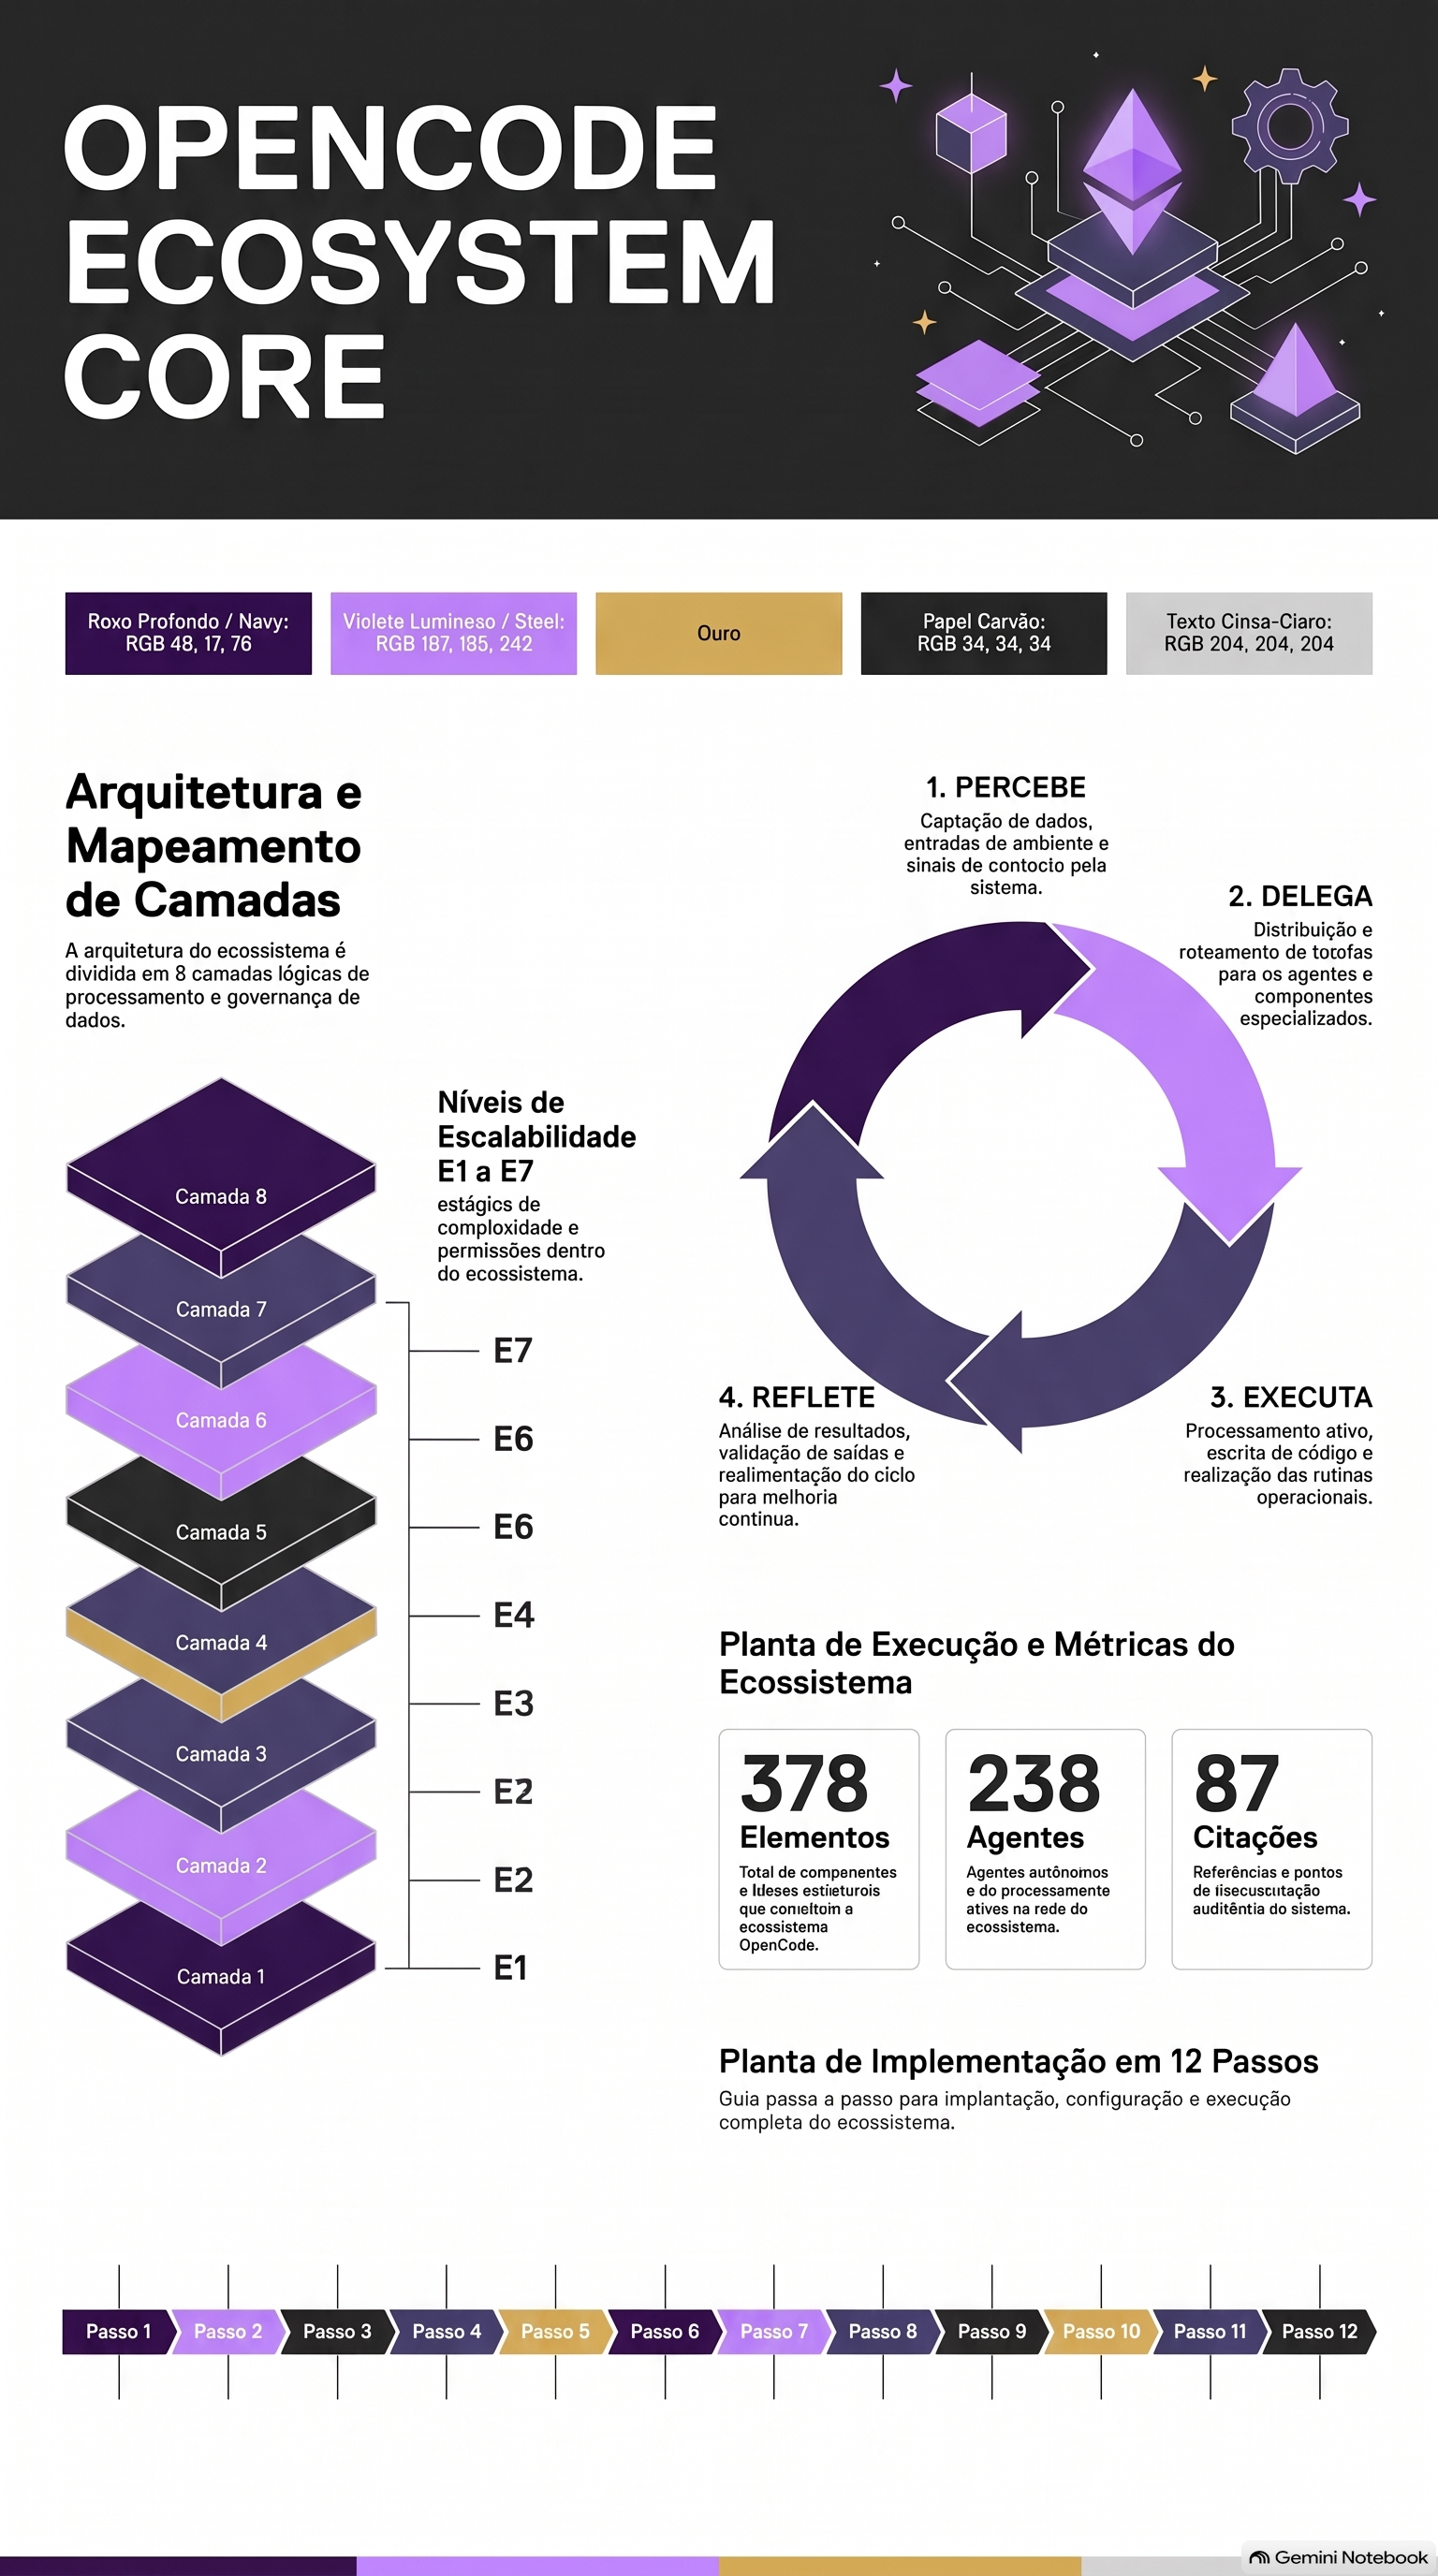
\includegraphics[width=0.92\textwidth]{fig-infografico-core.png}
\caption{Infogr\'afico do Core gerado no NotebookLM em pt-BR a partir da capa oficial: logotipo, paleta com RGB, 8 camadas, ciclo, m\'etricas e planta de 12 passos. Figura ilustrativa: microtextos podem conter trocas de letras do gerador; valem os n\'umeros do texto.}
\end{figure}

\begin{aviso}
Limite do atlas. Os dez mapas cobrem arququetipos por camada e por processo; fichas individuais do catalogo herdam o mapa da sua camada. Mapa algum substitui abrir o arquivo e rodar o comando.
\end{aviso}
